%--- Kapitel 8
\cleardoublepage
\chapter{Klassen und Objekte im Entwurf}
\label{sec:Kap-8}

In Kapitel~4 haben wir Klassen und Objekte im Rahmen der Domänenmodellierung betrachtet. Dort haben Sie das Klassendiagramm der UML kennengelernt. Im Rahmen des Entwurfs werden Klassen und Objekte nicht mehr nur aus dem Blickwinkel der Domäne betrachtet, sondern insbesondere aus dem Blickwinkel des zu realisierenden Softwaresystems. Trotzdem gilt weiterhin der Realweltbezug: ein großer Teil der zukünftigen Objekte des Softwaresystems ist von Objekten der Realwelt abgeleitet. Abhängig vom Einsatzzweck der Software werden bestimmte Eigenschaften der Realwelt-Objekte berücksichtigt und andere ignoriert, so dass nur die für die zukünftige Software relevanten Eigenschaften der Realwelt-Objekte betrachtet werden. Die so entstehenden Software-Objekte sind damit Abstraktionen von Realwelt-Objekten. 

Im Rahmen des Entwurfs wird überlegt, welche Software-Objekte benötigt werden und, davon ausgehend, welche entsprechenden Klassen nachher im Programmcode existieren sollen. Hierbei trifft man auf verschiedene Arten von Objekten:

\begin{itemize}
	\item Die schon bekannten Domänenobjekte, also diejenigen Software-Objekte, die auf Grundlage von Realweltentsprechungen der Domäne spezifiziert werden.
	\item Objekte, die im Rahmen der Benutzungsschnittstelle benötigt werden, zum Beispiel Bedienelemente wie Eingabefelder, Menüs, Buttons, Scrollbars, Comboboxen, Auflistungselemente, Checkboxen etc. Unabhängig davon, ob man die entsprechenden Klassen in seinem Softwareentwicklungsprojekt über\-wiegend selbst erstellt oder stärker auf vorhandene Klassenbibliotheken oder komplette GUI-Frameworks (GUI: Graphical User Interface, deutsch: grafische 
	\linebreak %%% für Druck
	Benutzungs\-oberfläche) zurückgreift, sind diese Objekte nachher Teil des entstandenen Softwaresystems.
	\item „Controller“-Objekte der Geschäftslogik. Hierunter fallen alle Objekte, die in Mechanismen zur Steuerung der fachlichen Abläufe der Software benötigt werden. Angenommen, im Zoobeispiel ist für das Tierinformationssystem vor\-gesehen, dass, wenn ein Nutzer das ihn interessierende Tier (z.B. den Hamster Paul) aus einer Liste aller Hamster des Zoos auswählt, er eine Detailseite mit Bildern und Informationen zu Hamster Paul angezeigt bekommt. Dort kann er dann noch einen Zeitraum für eine Patenschaft eintragen. Das System muss dafür im Hintergrund steuern, dass jeweils die richtigen \mbox{Informationen} \mbox{angezeigt} werden und bei der Patenschaft vielleicht prüfen, ob das Tier noch frei ist, die Kosten der Patenschaft ausrechnen, dann irgendwie noch mit dem Rechnungssystem des Zoos interagieren etc. Hierfür werden zusätzlich zu Domänen\-objekten wie Tier und Patenschaft und Oberflächenobjekten wie Liste und Beschreibungsseite Objekte bzw. deren Klassen benötigt, die diese Prozesse koordinieren.
	\item Objekte, die im Rahmen von Cross-Cutting Concerns wie Authentifizierungskomponenten oder Loggingmechanismen benötigt werden.
	\item Objekte, die aufgrund der Verwendung bestimmter Architektur- oder Entwurfs\-muster hinzukommen. Das sind häufig zusätzliche Abstraktionen und/oder Arten von Container-Objekten. Die Objektmengen aus diesem und dem vorherigen Aufzählungspunkt können sich durchaus überschneiden.
\end{itemize}
  
Für den Prozess der Implementierung müssen alle diese Objekte und ihre Beziehungen zueinander genau spezifiziert sein, denn sonst kann man den Programmcode nicht schreiben. In Softwareentwicklungsprojekten, die die Prozesse Entwurf und Implementierung strikt trennen, wird man diese Arbeit komplett auf der Ebene von grafischen Modellen oder textuellen Entwurfsbeschreibungen machen. Bei starker Verzahnung zwischen Entwurfs- und Implementierungstätigkeiten werden getroffene Entscheidungen dagegen teilweise auch direkt im Programmcode „dokumentiert“, indem entsprechende Klassen mit ihren Attributen und Operationsköpfen (die sogenannte Signatur, s. Lektion 6) sowie ggf. Kommentare dazu in der ausgewählten Programmiersprache angelegt werden.

Die folgenden Abschnitte knüpfen an die Vorstellung des UML-Klassendiagramms in Kapitel~4 an und stellen Elemente vor, die für Zwecke des Entwurfs benötigt werden. Eine komplette Übersicht der Elemente, die in einem UML-Klassendiagramm vorkommen dürfen, finden Sie bei \cite[37-118]{kec18}. 

\clearpage
\section{Attribute, Zustand und Identität}
\label{sec:Kap-8.1}

Ein Software-Objekt 
\marginline{Software-Objekt}
hat eine eindeutige Identität, die es von anderen Objekten unterscheidbar macht. Es besitzt Attribute, in denen seine Daten gespeichert sind, kann wechselnde Zustände annehmen und verfügt über eine Menge von Operationen, die sein Verhalten bestimmen. 

\vspace{2mm} %% für Druck

Attribute und Operationen von Objekten werden in den Klassen 
\marginline{Klasse}
definiert. In Kapitel~4 haben wir das Konzept Klasse aus dem Blickwinkel der Realweltmodellierung betrachtet. Danach ist eine Klasse die Beschreibung der Abstraktion von Realwelt-Objekt zu modelliertem Objekt. Aus dem Blickwinkel des zu erstellenden Softwareprodukts ist eine Klasse wieder eine Beschreibung, und zwar die Beschreibung von Struktur und Verhalten von Software-Objekten. 

\vspace{2mm} %% für Druck

Eine Klasse definiert, welche Attribute, welche Operationen und welche möglichen Beziehungen zu anderen Objekten die ihr zugehörigen Objekte aufweisen sollen. Eine Klasse definiert außerdem einen Mechanismus – in der objektorientierten Programmierung als \textit{Konstruktor} bezeichnet – über den neue Objekte vom Typ der Klasse erzeugt werden können. Jedes zur Laufzeit der Software benötigte Objekt einer Klasse wird so anhand der Vorgaben der Klasse konstruiert. Diese Erzeugung neuer Objekte einer Klasse nennt man \textit{Instanziierung} und statt vom Objekt der Klasse spricht man in diesem Zusammenhang von der \textit{Instanz}
\marginline{Instanzen}
(manchmal auch vom \textit{Exemplar}) der Klasse. Der Begriff Instanz wird verwendet, wenn die Zugehörigkeit zu seiner Klasse betont werden soll („Eine Instanz der Klasse Katze“), weil damit zum Beispiel ausgedrückt werden soll, dass diese konkrete Instanz alle Eigenschaften besitzt, die die entsprechende Klasse definiert hat. Der Begriff Objekt wird in allgemeineren Zusammenhängen eingesetzt. 

\vspace{2mm} %% für Druck

Die \textit{Identität}
\marginline{Identität}
eines Objekts besteht ab dem Zeitpunkt seiner Erzeugung und ist unveränderlich in der Lebenszeit des Objekts. In vielen Programmiersprachen ist die Speicheradresse des Objekts das Kriterium seiner Identität. 

\sttpDefinitionskasten{\sttpDefinitionskastenSkalierungsfaktor}{Zustand eines Objekts}{Die Gesamtheit der aktuellen Wertebelegungen aller seiner \mbox{Attribute}}{Es gibt noch eine erweiterte Definition, die auch die Verbindungen des Objekts umfasst, also: „Die Gesamtheit der aktuellen Wertebelegungen aller seiner Attribute sowie seine bestehenden Verbindungen zu anderen Objekten.“ Die kurze Defini\-tion, die auch wir hier verwenden, entstammt einem implementierungsnahen Blickwinkel. Im Rahmen der Implementierung werden auch die Verbindungen zwischen Objekten auf Attribute abgebildet -- allerdings nicht zwingend auf Attribute dieses Objekts. Insofern sind es durchaus zwei unterschiedliche Defini\-tionen von Objektzustand.}

\clearpage %%% für Druck

Der \textit{Zustand} eines Objekts definiert sich über die Wertebelegungen seiner Attribute zum aktuellen Zeitpunkt. Daraus ergibt sich, dass sich der Zustand eines Objekts ändert, wenn sich mindestens der Wert eines seiner Attribute ändert. Unabhängig davon, wie häufig sich der Zustand eines Objekts in seiner Lebenszeit ändert, die Identität des Objekts ändert sich niemals. 

\vspace{2mm} %% für Druck

Wir 
\marginline{Identität vs. Zustand}
verdeutlichen die Konzepte Identität und Zustand an einem Beispiel. Abbildung~\ref{fig:identitaet_vs_zustand} schließt an das Autobeispiel aus Abschnitt~4.2 an und zeigt Auto-Objekte mit den beiden Attributen \sttpUMLText{modell} und \sttpUMLText{farbe}. Links sehen Sie das Objekt 
\linebreak %%% für Druck
\sttpUMLText{ellensAuto} mit dem Wert stahlblau im Attribut \sttpUMLText{farbe}. Ganz rechts sehen Sie ein anderes Objekt, nämlich das Objekt \sttpUMLText{heikesAuto} mit dem Wert rot im Attribut \sttpUMLText{farbe}. Es soll sich um zwei verschiedene Objekte handeln, jedes mit seiner eigenen Identität. In der Mitte der Abbildung betrachten wir erneut das Objekt \sttpUMLText{ellensAuto}, allerdings zu einem späteren Zeitpunkt als zum Zeitpunkt des linken Teils der Abbildung. Wir nehmen an, dass \sttpUMLText{ellensAuto} zu diesem zweiten Zeitpunkt umlackiert ist. Der Wert im Attribut \sttpUMLText{farbe} ist jetzt nicht mehr stahlblau, sondern rot. Durch die Änderung in diesem einem Attribut ändert sich der Zustand des Objekts \sttpUMLText{ellensAuto}, seine Identität aber nicht. Die Abbildungen links und in der Mitte beziehen sich also auf dasselbe Objekt.

\begin{figure}[h!]
	\centering
	\includegraphics[scale=1.0]{Bilder/Kapitel-8/identitaet_vs_zustand.pdf}
	\vspace{\baselineskip} %% für Druck
	\caption[Zustand und Identität]{Ein Objekt zum Zeitpunkt t1 (links), dasselbe Objekt zum Zeitpunkt t2 in einem anderen Zustand (Mitte) und ein Objekt mit anderer Identität (rechts)}
	\label{fig:identitaet_vs_zustand}
\end{figure}

\sttpUMLText{ellensAuto} in der Mitte und \sttpUMLText{heikesAuto} rechts stimmen in den Wertebelegungen der beiden Attribute \sttpUMLText{modell} und \sttpUMLText{farbe} überein. Sie haben denselben Zustand, aber nicht dieselbe Identität. Die Änderung der Wertebelegung der Attribute eines Objekts hat keine Auswirkungen auf andere Objekte der Klasse. \sttpUMLText{heikesAuto} bleibt rot, auch wenn wir die Farbe von \sttpUMLText{ellensAuto} erneut ändern. Die beiden Objekte sind dann nur nicht mehr zustandsgleich.

\vspace{2mm} %% für Druck

Von der Zustandsgleichheit 
\marginline{Zustands\-gleichheit und referentielle Gleichheit}
zu unterscheiden, ist die sogenannte referentielle Gleichheit. Referentielle Gleichheit liegt vor, wenn sich hinter zwei unterschiedlichen 
\linebreak %%% für Druck
Objektnamen das identische Objekt verbirgt, es sich also nur um zwei Referenzen auf dasselbe Objekt handelt. Betrachten Sie Abbildung~\ref{fig:zustands_referentielle_gleichheit}.

\begin{figure}[h!]
	\centering
	\includegraphics[scale=1.0]{Bilder/Kapitel-8/zustands_referentielle_gleichheit.pdf}
	\caption{Zustandsgleichheit und referentielle Gleichheit}
	\label{fig:zustands_referentielle_gleichheit}
\end{figure}

\pagebreak %%% für Druck

Links sind drei Auto-Objekte abgebildet: \sttpUMLText{ellensAuto}, \sttpUMLText{heikesAuto} und 
\linebreak %%% für Druck
\sttpUMLText{frauMeyersAuto}. Alle drei Objekte sind zustandsgleich. Wir ändern den Wert im Attribut \sttpUMLText{farbe} in \sttpUMLText{ellensAuto} von rot zu grün und erhalten die drei Objekte in den rechts abgebildeten Zuständen: \sttpUMLText{ellensAuto} ist grün, \sttpUMLText{heikesAuto} weiterhin rot, aber \sttpUMLText{frauMeyersAuto} plötzlich auch grün. Warum? Die Erklärung ist, dass es sich bei \sttpUMLText{ellensAuto} und \sttpUMLText{frauMeyersAuto} offensichtlich nicht um zwei unterschiedliche Objekte, sondern um dasselbe Objekt handelt, das in unserem Diagramm nur mit unterschiedlichen Namen gekennzeichnet wurde. Der Objektname ist nie gleichzusetzen mit der Identität des Objekts. Der Name ist lediglich ein Bezeichner, der das Objekt im Kontext (\zb im Diagramm, im Programmcode) identifiziert.

\vspace{2mm} %% für Druck

Manche 
\marginline{readOnly}
Eigenschaften von Realwelt-Objekten, wie zum Beispiel der Modelltyp \mbox{eines} Autos, ändern sich nicht. Bei der Abbildung einer Eigenschaft auf ein Software-Objekt möchte man eine solche Unveränderlichkeit vielleicht auch ausdrücken können. Die UML bietet dafür die textuelle Ergänzung \sttpUMLText{\{readOnly\}} an, die in der Klasse hinter dem Attribut notiert wird. Ein Beispiel dafür sehen Sie weiter hinten im Text in Abbildung~\ref{fig:klasse_auto_getter_setter}. Die Klasse Auto müsste dann natürlich später auch so implementiert werden, dass sichergestellt ist, dass jede Auto-Instanz einen Attributwert für \sttpUMLText{modell} enthält, dieser Wert aber während der Lebenszeit der Instanz nicht verändert werden kann. 
\clearpage
\section{Operationen}
\label{sec:Kap-8.2}

In der objektorientierten Softwareentwicklung ist ein Objekt eine Einheit aus \mbox{Daten} und den Operationen, die mit diesen Daten arbeiten. Die Daten werden in den Attri\-buten gespeichert und können sich – abgesehen von Zustandsgleichheit – bei den unterschiedlichen Instanzen der Klasse auch unterscheiden. Bei den Operationen ist das anders. Die Operationen, die das Verhalten der Objekte bestimmen, sind für alle Instanzen einer Klasse identisch. Die UML bietet dementsprechend auch keine Möglichkeit, Operationen in Objekten zu modellieren, sondern nur in der zugehörigen Klasse.

Abbildung~\ref{fig:klasse_auto} zeigt die UML-Darstellung der Auto-Klasse mit den Attributen 
\linebreak %%% für Druck
\sttpUMLText{modell} und \sttpUMLText{farbe} ergänzt um die Operation \sttpUMLText{lackieren}. Für die Darstellung von Operationen wird das Rechteck der Klasse erneut horizontal unterteilt. Wie die Attri\-bute werden die Operationen linksbündig untereinander aufgeführt. 

\vspace{\baselineskip} %%% für Druck

\begin{figure}[h!]
	\centering
	\includegraphics[scale=1.0]{Bilder/Kapitel-8/klasse_auto.pdf}
	\caption{Die Klasse \sttpUMLText{Auto} mit zwei Attributen und einer Operation}
	\label{fig:klasse_auto}
\end{figure}

Die Operationen einer Klasse spezifizieren, welche Funktionalität die Instanzen dieser Klasse anderen Objekten des Systems anbieten – technisch gesprochen: welche Funktionalität in welcher Weise aufgerufen werden kann. Man verwendet in diesem Zusammenhang auch den Begriff Dienstleistung
\marginline{Dienstleister, Dienstnutzer}
und beschreibt mit den Begriffen Dienstleister und Dienstnutzer -- die wir in Kapitel~\ref{sec:Kap-7} schon häufiger verwendet hatten --, welche Rolle ein Objekt bei Ausführung einer bestimmten Operation einnimmt. Das Objekt, das eine Operation aufruft, ist der Dienstnutzer und das Objekt, dessen Operation aufgerufen wird, ist der Dienstleister. Die entsprechende Operation (bzw. die Funktionalität, die sie abbildet) ist dementsprechend der Dienst. 

Die reine objektorientierte Modellierung abstrahiert eigentlich von dieser technischen Ebene der Operationsaufrufe und verwendet die Metapher
\marginline{Metapher\\ Nachrichten\-versand}
des Nachrichtenversands bzw. des Austauschens von Botschaften zwischen Objekten: Ein Objekt sendet eine Nachricht an ein anderes Objekt. Das die Nachricht empfangende Objekt reagiert entweder entsprechend seiner definierten Verhaltensweisen oder reagiert nicht, wenn es für die Nachricht keine definierten Verhaltensweisen besitzt. Das Konzept des Nachrichtenaustausches zwischen Objekten orientiert sich an der Realwelt: Realwelt-Objekte übermitteln verbal oder nonverbal Botschaften an andere Realwelt-Objekte (\zb die Aufforderung einer Mutter an ihr Kind, das Zimmer aufzuräumen oder der fast-verhungernde Blick eines Hundes zu seinem Besitzer) und diese reagieren auf bestimmte Art und Weise. Der Austausch von Nachrichten zwischen den Objekten in einem Softwaresystem bleibt letztendlich aber doch eine Folge von Operationsaufrufen und Operationsausführungen. Die Nachricht des Sender-Objekts besteht aus einem Operationsnamen und gegebenenfalls zusätzlichen Informationen in Form von Parametern (\su). Das Empfänger-Objekt kann auf diese Nachricht genau dann reagieren, wenn dafür eine entsprechende Operation definiert ist.\footnote{Objektorientierte Programmiersprachen verlangen in der Regel, dass nur Nachrichten gesendet werden, auf die ein Objekt auch reagieren kann. In compilierten Sprachen achtet darauf schon der Compiler. In Interpreter-Sprachen lösen Nachrichten, auf die nicht reagiert werden kann, Laufzeitfehler aus. Der Fall, dass ein Objekt eine Nachricht nicht verstehen kann, wird also im Gegensatz zur Realwelt nicht als gültige Möglichkeit angesehen.} Die Ausgestaltung der Operation bestimmt, was genau bei Eintreffen der Nachricht des Sender-Objekts passiert. 

Wir führen Operationen erst hier ein, in der Lektion zum Thema Entwurf. Das heißt aber nicht, dass man nicht auch in Domänenklassendiagrammen schon Operationen finden kann. Insbesondere in einer unspezifizierten Darstellungsform wie in Abbildung~\ref{fig:klasse_auto}, nur mit Operationsnamen und leerer Parameterliste, also ohne Parameter und ohne Angabe von Datentypen, kann man sie gut auch für Diskussionen mit den Kunden einsetzen. 

Im
\marginline{Parameter und Datentypen}
Rahmen des Entwurfs des Softwareprodukts benötigt man detailliertere Informa\-tionen zu den Operationen, da man diese sonst später nicht als Programmcode umsetzen kann. Abbildung~\ref{fig:klasse_auto_detailliert} zeigt eine erweiterte Darstellung der Auto-Klasse mit verschiedenen Möglichkeiten Parameter, Datentypen und Vorgabewerte anzugeben. Wir vermischen in dieser Abbildung verschiedene Abstraktionsebenen, um alle Aspekte an dieser einen Abbildung zeigen zu können. Eine echte Klasse sollte so nicht aussehen.

\begin{figure}[h!]
	\centering
	\includegraphics[scale=1.0]{Bilder/Kapitel-8/klasse_auto_detailliert.pdf}
	\caption[Die Klasse \sttpUMLText{Auto} mit detaillierteren Informationen]{Die Klasse \sttpUMLText{Auto} mit detaillierteren Informationen zu Attributen und Operationen}
	\label{fig:klasse_auto_detailliert}
\end{figure}

\pagebreak %%% für Druck

Attributnamen können um den Datentyp des Attributs (Attributtyp) ergänzt werden. Dazu wird in der UML-Darstellung hinter dem Attributnamen ein Doppelpunkt und dann der Attributtyp ergänzt. Zusätzlich kann nach dem Attributtyp auch noch ein Vorgabewert (default value) angegeben werden (wie bei \sttpUMLText{füllstandTank}). Ein Vorgabewert ist die Wertebelegung, die ein Objekt bei seiner Erzeugung erhalten soll.

Bei den Operationen können Übergabeparameter und Rückgabetypen aufgeführt werden. Die Parameter werden in gleicher Weise wie die Attribute mit Namen und Datentyp innerhalb der runden Klammern der Parameterliste der Operation angegeben. Wenn eine Operation mehrere Parameter hat, werden diese mit Komma getrennt. Je nachdem, wie implementierungsnah ein Diagramm sein soll, handelt es sich bei den Attribut- und Parametertypen schon um programmiersprachliche Datentypen (wie int und String in der Abbildung) oder noch um domänen- oder allgemeinsprachliche Angaben (wie Farbe und Liter). Gerade in Klassen\-diagrammen, die für die Kommunikation mit Nicht-Programmierern gedacht sind, finden sich häufiger Angaben wie Euro, Liter, Farbe, Grad Celsius etc. statt Integer, Float, String. Die beiden Ebenen zu mischen, wie in dieser Abbildung, ist aber eigentlich nicht sinnvoll. 

Verbund-Datentypen, die mehrere Elemente enthalten, wie Arrays oder Listen, 
\linebreak %%% für Druck
lassen sich in UML auch modellieren, allerdings in einer verallgemeinerten Form 
\linebreak %%% für Druck
über Multiplizitäten, da die UML versucht, von den verschiedenen Daten-
\linebreak %%% für Druck
strukturen konkreter Programmiersprachen zu abstrahieren. Über die Angabe 
\linebreak %%% für Druck
\sttpUMLText{[untereGrenze..obereGrenze]} lässt sich ein Datentyp entsprechend ergänzen. So bedeutet eine Angabe \sttpUMLText{int[1..5]}, dass es sich um \textbf{irgendeinen} Verbund-Datentypen handelt, in dem ein bis fünf Integer-Elemente enthalten sind. Weiter hinten im Text, in Abbildung~\ref{fig:klassen_tier_und_gehege}, wird ein solcher Datentyp verwendet. Wenn es sich um ein sehr implementierungsnahes Entwurfsdiagramm handelt und man die genaue Datenstruktur schon festlegen möchte, kann man zusätzlich mit textuellen Ergänzungen in geschweiften Klammern arbeiten. 

Ein weiterer Datentyp sind Enumerations. Eine Enumeration ist ein Datentyp mit endlichem Wertebereich, der in vielen Programmiersprachen vorkommt. Enumerations funktionieren als Aufzählungstypen, indem sie die möglichen Werte in einer Aufzählungsform angeben. Abbildung~\ref{fig:enumeration_farbe} zeigt ein Beispiel. 

\begin{figure}[h!]
	\centering
	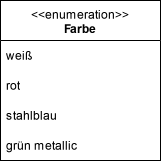
\includegraphics[scale=1.0]{Bilder/Kapitel-8/enumeration_farbe.pdf}
	\caption{Datentyp Enumeration}
	\label{fig:enumeration_farbe}
\end{figure}

\pagebreak %%% für Druck

Die UML stellt Enumerations in einer klassenähnlichen Form dar. In vielen Programmiersprachen sind Enumerations tatsächlich auch als Klassen realisiert (in \mbox{Java} auch). Das Stichwort \sttpUMLText{<<enumeration>>} in der ersten Zeile -- in UML Begriffen heißen diese \sttpUMLText{<<...>>}~-~Konstruktionen Stereotype -- signalisiert, dass es sich um eine Enumeration handelt. Die möglichen Werte werden wie die Attribute einer Klasse untereinander aufgeführt. 

\vspace{2.5mm} %%% für Druck

In der Auto-Klasse in Abbildung~\ref{fig:klasse_auto_detailliert} gab es ein Attribut \sttpUMLText{farbe : Farbe}, bei dessen Datentyp \sttpUMLText{Farbe} es sich um einen allgemeinsprachlichen Datentyp handelte. Genau auf diese Weise würde auch ein Enumerations-Datentyp angegeben, nur sollte sich dann die Information zur Enumeration (also Abbildung~\ref{fig:enumeration_farbe}) ebenfalls im Diagramm befinden bzw. anderweitig bekannt sein. Ansonsten kann dem Leser des Modells unklar bleiben, ob hier ein allgemeinsprachlicher Datentyp, eine Enumeration als Datentyp oder ein Objekt der Klasse \sttpUMLText{Farbe} -- das wird nämlich ebenso notiert -- gemeint ist.

\vspace{2.5mm} %%% für Druck

Wie detailliert (und auch wie implementierungsnah in den Bezeichnungen) ein 
\linebreak %%% für Druck
Klassendiagramm des Entwurfs ist, hängt einerseits davon ab, zu welchem Zweck es eingesetzt werden soll. Klassendiagramme, anhand derer Programmierer schon die konkrete Klassenstruktur in der Programmiersprache anlegen sollen, müssen deutlich detaillierter sein als Klassendiagramme, die als Diskussionsgrundlage über den Entwurf der Software gedacht sind. Andererseits hängt der benötigte Detailgrad \mbox{eines} Entwurf-Klassendiagramms auch davon ab, in welchem Ausmaß Artefakte aus dem Prozess des Requirements Engineering (textuelle Beschreibungen oder andere Arten von Diagrammen) vorhanden sind. Es ist zum Beispiel nicht zwingend, eine modellierte Klasse im Klassendiagramm mit allen Details auszustatten, wenn zu derselben Klasse auch eine für den Entwurf angemessene, detaillierte textuelle Beschreibung vorliegt.

\vspace{2.5mm} %%% für Druck

Wir kommen zum Thema Operationen zurück. Wie gesehen, werden die Opera\-tionen in den Klassen definiert. Zur Laufzeit des Programms werden sie dann aber auf \mbox{einem} konkreten Objekt aufgerufen. In Reaktion auf den Aufruf einer Operation zeigt dieses Objekt dann ein bestimmtes Verhalten. Dabei kann es sich auch um die Änderung seines Zustands handeln, zum Beispiel wenn in der Spezi\-fika\-tion der Operation \sttpUMLText{lackieren} steht, dass der Wert des Attributs \sttpUMLText{farbe} durch den Wert des übergebenen Parameters \sttpUMLText{neueFarbe} ersetzt werden soll. Die Reaktion auf einen Operations\-aufruf kann abhängig vom Zustand des Objekts, auf dem der Operationsaufruf durchgeführt wird, sowie abhängig von den durch das aufrufende Objekt übergebenen Parametern unterschiedlich ausfallen. So ist es zum Beispiel sinnvoll, wenn eine Auto-Instanz, deren Tank leer ist, auf einen Operationsaufruf \sttpUMLText{tanken(30 Liter)} anders reagiert als eine andere Auto-Instanz, deren Tank komplett gefüllt ist. 

\vspace{2.5mm} %%% für Druck

Man
\marginline{Selektoren, Modifikatoren}
unterscheidet Operationen, die nur lesend auf Attribute zugreifen und deren Werte nicht verändern (Selektoren) und solche, die Attributwerte verändern, also (auch) schreibend auf Attribute zugreifen (Modifikatoren). Modifikatoren ändern also den Zustand eines Objekts, Selektoren tun dies nicht. Die Operation \sttpUMLText{lackieren} ist ein Beispiel für einen Modifikator. 

\pagebreak %%% für Druck

\vspace*{\baselineskip} %%% für Druck

\begin{figure}[h!]
	\centering
	
\includegraphics[scale=1.0]{Bilder/Kapitel-8/klasse_thermometer.pdf}
	\caption{Eine Selektor-Operation}
	\label{fig:klasse_thermometer}
\end{figure}

\vspace{\baselineskip} %%% für Druck

Abbildung~\ref{fig:klasse_thermometer} zeigt ein Beispiel für eine Selektor-Operation: Die Klasse \sttpUMLText{Thermometer} besitzt ein Attribut \sttpUMLText{temperatur}, das die Temperatur in der Einheit Grad Celsius enthält. Die Operation \sttpUMLText{berechneFahrenheit()} liest diesen Wert aus und errechnet daraus die Temperatur in der Einheit Grad Fahrenheit. In der UML können Selektor-Operationen durch den Zusatz \sttpUMLText{\{isQuery\}} gekennzeichnet werden. Dieser Zusatz ist aber optional. Für manche Modellierungszwecke im Laufe der Softwareentwicklung ist es nicht relevant, ob eine bestimmte Operation in der späteren konkreten Implementierung ein Selektor oder ein Modifikator werden soll.

\vspace{2mm} %%% für Druck

Die
\marginline{Getter, Setter}
„einfachsten“ Selektor- und Modifikator-Operationen sind die (eingedeutscht sogenannten) Getter und Setter. Eine get-Operation liest den Wert eines bestimmten Attributs aus und liefert diesen zurück. Eine set-Operation nimmt über einen Parameter einen Wert entgegen und ersetzt den aktuellen Wert eines bestimmten Attributs durch den Parameterwert. 

\vspace{\baselineskip} %%% für Druck
\vspace{3mm} %%% für Druck

\begin{figure}[h!]
	\centering
	\includegraphics[scale=1.0]{Bilder/Kapitel-8/klasse_auto_getter_setter.pdf}
	\caption{get-Operationen und set-Operationen} % hier absichtlich die Kleinschreibung behalten
	\label{fig:klasse_auto_getter_setter}
\end{figure}

\vspace{\baselineskip} %%% für Druck

Abbildung~\ref{fig:klasse_auto_getter_setter} zeigt eine Klasse \sttpUMLText{Auto} mit einer get- und einer set-Operation für das Attribut \sttpUMLText{farbe}. Da das Attribut \sttpUMLText{modell} nicht veränderlich sein soll, wird für dieses Attribut keine set-Operation angelegt. Um ein Klassendiagramm nicht zu überladen, werden die Getter und Setter häufig nicht aufgeführt – oft auch in sehr implementierungs\-nahen Klassendiagrammen nicht. Die Information, zu welchen Attri\-buten einer Klasse es Getter bzw. Setter geben soll und zu welchen nicht, muss allerdings im Softwareentwicklungsteam dann anderweitig entschieden und bekannt gemacht werden.

\vspace{2mm} %%% für Druck

Get- und set-Operationen zu verwenden, anstatt auf die Attribute des Objekts \mbox{direkt} zuzugreifen, ist ein erster Schritt zur Einhaltung des Geheimnisprinzips 
\linebreak %%% für Druck
(s.~Kap.~\ref{sec:Kap-7.2.1}). Im Sinne des Geheimnisprinzips wäre es noch besser, das Wissen über vorhandene Attribute weiter zu verbergen, indem nicht mit jedem einzelnen Attribut gearbeitet, sondern auf die zu erbringende Dienstleistung fokussiert und diese über entsprechende Operationen zur Verfügung gestellt wird. Zum Beispiel würde eine Operation, die lackieren heißt (\sttpUMLText{lackieren(neueFarbe : Farbe)}), dem inhaltlichen Zweck Farbänderung aus Dienstnutzersicht erstens viel eher entsprechen als den Auftrag zu geben, ein bestimmtes Attribut zu ändern. Zweitens läge es in der Hoheit der Klasse \sttpUMLText{Auto}, diese lackieren-Operation weiter auszugestalten als nur das Attribut \sttpUMLText{farbe} zu ändern, zum Beispiel indem in einem anderen Attribut die alte Farbe des Autos dokumentiert wird oder indem der letzte Lackierungszeitpunkt gelesen wird und dementsprechend einfach oder doppelt lackiert wird etc. Den Dienstnutzer braucht nicht zu interessieren, welche Attribute wie verändert werden, solange das Auto am Ende die gewünschte neue Farbe hat. Technisch könnte man diese ganzen Dinge natürlich auch in einer setFarbe-Operation unterbringen, aber das verringert das Verständnis des Programmcodes enorm, weil niemand in einem Setter für das Attribut \sttpUMLText{farbe} anderes als eine Änderung dieses Attributs erwarten würde. 

\vspace{2mm} %%% für Druck

Wenn man jetzt noch eine Spur mehr abstrahieren möchte, folgt man den Entwurfs\-prinzipien für Schnittstellen und lässt die lackieren-Operation nicht direkt auf der Klasse \sttpUMLText{Auto}, sondern auf einer zugehörigen Schnittstelle aufrufen. Man kann aller\-dings auch Komplexität erzeugen, indem man übermäßig abstrahiert. Insofern haben Getter und Setter in jedem Fall ihre Berechtigung -- und werden auch häufig verwendet --, auch wenn sie weniger von den Implementierungsdetails einer Klasse verbergen als es mit anderen Konstruktionen möglich wäre.

\vspace{\baselineskip} %%% für Druck
\vspace{1mm} %%% für Druck

\minisec{Währenddessen im Zoo}
Wir nehmen an, im Zooprojekt ist Folgendes geschehen:

Im Prozess des Requirements Engineering hat man sich darauf verständigt, dass es zukünftig zu den Aufgaben der Tierpfleger gehören wird, die Daten der neugeborenen Tiere zu erfassen, damit diese über das Tierinformationssystem auf der Zoo-Website der Öffentlichkeit zugänglich gemacht werden können. Über ein Anwendungsfall\-diagramm wurde schon etwas differenzierter festgehalten, was ein Tierpfleger dafür mit dem Softwaresystem tun können muss (Abbildung~\ref{fig:neugeborene_tiere_erfassen}).

\begin{figure}[h!]
	\begin{addmargin*}[0cm]{-\marginparwidth}
	\begin{addmargin*}[0cm]{-\marginparsep}
		\vspace{\baselineskip} %%% für Druck
		\centering
		\includegraphics[scale=0.9]{Bilder/Kapitel-8/neugeborene_tiere_erfassen.pdf}
		\caption{Anwendungsfall "`neugeborene Tiere erfassen"'}
		\label{fig:neugeborene_tiere_erfassen}
	\end{addmargin*}
	\end{addmargin*}	
\end{figure}

Jetzt im Entwurfsprozess wurden die grundsätzliche Softwarearchitektur für das Tier\-informations\-system festgelegt und auch schon einige Entscheidungen zum Aussehen der Benutzungsoberfläche getroffen. Auf Grundlage aller dieser Ergebnisse ist folgende textuelle Beschreibung für den Prozess "`neugeborene Tiere erfassen"' entstanden.

\sttpUniversalkasten{Erfassung neugeborener Tiere}{
	\phantomsection
	\label{sec:Kap-8.2:Tiererfassung}
		
	Der Tierpfleger ruft die Maske \sttpUMLText{Tiererfassung} auf, um die Daten eines neugeborenen Tiers einzugeben. Er trägt in die entsprechenden Formularfelder die Stammdaten zum Tier (Name, Geburtsdatun, Größe, Gewicht) ein. Er kann auch schon eine Beschreibung der Besonderheiten des Tiers im Vergleich zu anderen Tieren derselben Art eintragen. Diese Informationen können aber auch später nachgetragen werden. Er wählt die Tierart über eine Dropdown-Liste aus. Die Eltern des Tiers wählt er über ein kontextsensitives Suchfeld mit Autovervollständigungsfunktion (freie Eingabe von Text, als Suchvorschläge werden nur Tiere derselben Tierart angegeben) aus. Er speichert die ausgefüllte Erfassungsmaske. Als letzten Schritt wechselt er auf die Übersichtsseite der Gehege und wählt dort das Gehege aus, in dem das neugeborene Tier wohnen wird. Über die Bearbeitungsfunktion auf der entsprechenden Gehege-Detailseite fügt er dem Gehege das neue Tier hinzu (anhand der aus dem vorherigen Schritt gemerkten Tier-ID oder per Auswahl aus einer Tierart-spezifischen Auswahlliste).}

\pagebreak %%% für Druck

Wir verlassen den Zoo und wechseln zurück auf die Metaebene: Aus einer solchen Beschreibung ergeben sich Objekte, deren zugehörige Klassen im Klassendiagramm berücksichtigt werden müssen. Von den Domänenobjekten sind das Tier, Gehege und Tierart. Potenzielle Kandidaten für Objekte der Benutzungsoberfläche sind Erfassungs\-maske oder Dropdown-Liste. Aber welche von denen dann schluss\-endlich durch Klassen repräsentiert werden, welche nur durch Attribute von anderen, welche reine Views sind etc., ist stark abhängig davon, mit welcher "`Technologie"' man die Benutzungsoberfläche umsetzt (selbst programmiert, über ein bestimmtes GUI-Framework, über reine HTML-Formularelemente etc.). Wir bleiben hier bei den Domänenobjekten. Für die Klasse \sttpUMLText{Tier} finden sich eine Reihe von benötigten Attri\-buten. Abbildung~\ref{fig:klasse_tier} zeigt die Klasse \sttpUMLText{Tier} mit diesen Attributen. Wir kommen auf verschiedene Aspekte dieser Tierklasse in den folgenden Abschnitten zurück. 

\vspace{\baselineskip} %%% für Druck

\phantomsection
\label{sec:Kap-8.2:Tierklasse}

\begin{figure}[h!]
	\centering
	\includegraphics[scale=1.0]{Bilder/Kapitel-8/klasse_tier.pdf}
	\caption{Eine Klasse \sttpUMLText{Tier}}
	\label{fig:klasse_tier}
\end{figure}
\clearpage
\section{Klassenattribute und Klassenoperationen}
\label{sec:Kap-8.3}

Bisher haben wir Attribute betrachtet, die zwar durch die Klasse definiert werden, für die aber jede Instanz der Klasse ihre eigenen Wertebelegungen haben kann. Das Klassenkonzept der Objektorientierung sieht neben diesen Attributen, die man auch Instanzattribute nennen kann, noch eine andere Art von Attributen vor, die sogenannten \textit{Klassenattribute}. Ein Klassenattribut ist ein Attribut, das in der Klasse verortet ist und dessen Wert von allen Instanzen der Klasse geteilt wird. Im Unter\-schied zu Instanzattributen besitzt also nicht jede Instanz eine eigene Wertebelegung für dieses Attribut, sondern es existiert nur ein gemeinsamer Wert. Wird dieser Wert verändert, haben alle Instanzen der Klasse eine neue Wertebelegung in dem entsprechenden Attribut. Klassenattribute verwendet man für die Abbildung von Eigenschaften, die relevant für die inhaltliche Modellierung einer konkreten \mbox{Klasse} sind, sich aber nicht den einzelnen Instanzen der Klasse zuordnen lassen. Ein Klassen\-attribut existiert auch dann, wenn (noch) keine Instanz der Klasse erzeugt wurde. 

\vspace{\baselineskip} %%% für Druck
\vspace{2mm} %%% für Druck

\begin{figure}[h!]
	\centering
	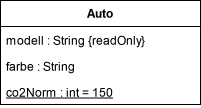
\includegraphics[scale=1.0]{Bilder/Kapitel-8/klasse_auto_mit_klassenattribut.pdf}
	\caption{Klassenattribut}
	\label{fig:klasse_auto_mit_klassenattribut}
\end{figure}

\vspace{2mm} %%% für Druck

Ein Klassenattribut in unserem Autobeispiel-Kontext könnte \sttpUMLText{co2Norm} sein, wenn wir idealisiert annehmen, dass für alle Automodelle eine einheitliche $\text{CO}_2$-Abgasnorm gilt (Abb.~\ref{fig:klasse_auto_mit_klassenattribut}). Klassenattribute werden in der UML-Darstellung der Klasse unter\-strichen. In der Darstellung der Instanzen wird ein Klassenattribut identisch zu den Instanzattributen dargestellt, also nicht unterstrichen. Häufig wird ein Klassen\-attribut aber aus Redundanzgründen (da es für jede Instanz denselben Wert hat) gar nicht in der Darstellung der Instanzen aufgeführt. Neben den Klassen\-attributen gibt es auch \textit{Klassenoperationen}. Klassenoperationen werden auf der Klasse und nicht auf einer konkreten Instanz aufgerufen. Sie werden verwendet, um auf die Klassenattribute zuzugreifen. Wie die Klassenattribute werden Klassenoperationen in der UML-Darstellung unterstrichen.

\vspace{2mm} %%% für Druck

Eine 
\marginline{Konstruktoren, Destruktoren}
besondere Form von Operationen sind die Operationen zum Erzeugen und Löschen von Instanzen, die sogenannten Konstruktoren und Destruktoren. In manchen objektorientierten Programmiersprachen entspricht ihre Syntax der Syntax von Klassenoperationen. In Java haben Konstruktoren eine spezielle Syntax, die sich von derjenigen der Klassenoperationen unterscheidet. Zudem kennt Java keine Destruktoren, sondern stattdessen das Konzept des Garbage Collectors, nicht mehr verwendete Instanzen werden automatisch gefunden und zerstört. Konstruktoren und Destruktoren werden aus Übersichtlichkeitsgründen üblicherweise nicht im UML-Klassendiagramm aufgeführt.
\clearpage
\section{Navigierbarkeit}
\label{sec:Kap-8.4}

Die UML bietet die Möglichkeit, (Klassen)Assoziationen und (Objekt)Verbindungen mit Navigierbarkeiten zu versehen. Dafür werden die Enden der Linien zwischen den Klassen bzw. Objekten um Pfeilspitzen ergänzt. Die Navigierbarkeit erlaubt es, die Interaktion zwischen den Objekten und die Rollen, die Objekte einnehmen können (Dienstleister und/oder Dienstnutzer) genauer zu spezifizieren. Die UML unterscheidet zwischen
\begin{itemize}
	\item \textit{navigierbar}, mit den Formen
	\begin{itemize}
		\item \textit{unidirektional navigierbar} und 
		\item \textit{bidirektional navigierbar}, 
	\end{itemize}
	\item \textit{nicht navigierbar} und
	\item \textit{unspezifiziert}.
\end{itemize}

Die Navigierbarkeit einer Beziehung sagt aus, inwiefern sich die verbundenen Elemente kennen oder nicht kennen, also je nach Metapher: sich Nachrichten schicken können, als Dienstleister auftreten können, Operationen des anderen aufrufen können. Wenn ein Objekt ein anderes Objekt kennt, kann es dessen Dienstleistungen nutzen, indem es Operationen des anderen Objekts aufruft. Auf einer implemen\-tierungs\-technischen Ebene bedeutet Navigierbarkeit, dass ein Objekt einer Klasse~A, die Klasse~B kennt, ein Attribut vom Datentyp der Klasse B besitzt. 

Die Verbindungen und Assoziationen in den Abbildungen in Kapitel~4
(durchgezogene Linien ohne Pfeilspitzen) waren bezüglich der Navigierbarkeit alle unspezifiziert. Unspezifiziert bedeutet, dass wir uns zum Erstellungszeitpunkt des Klassen\-diagramms noch keine Gedanken darüber gemacht haben, ob zum Beispiel (Abb.~4.12 in Kap.~4) % TODO (Abb.~\ref{fig:klassendiagramm_zu_objektdiagramm} in Kap.~\ref{sed:Kap-3}) 
eine Lehrer-Instanz Operationen einer Fach-Instanz aufrufen können soll und/oder umgekehrt. In Domänenklassendiagrammen findet man häufig noch unspezifizierte Navigierbarkeiten. Im Laufe von Entwurfsaktivitäten oder spätestens während der Implementierung müssen Navigierbarkeitsentscheidungen getroffen werden. 

\vspace{\baselineskip} %%% für Druck

\begin{figure}[h!]
	\centering
	\includegraphics[scale=1.0]{Bilder/Kapitel-8/navigierbarkeiten_gast_restaurant.pdf}
	\caption{Navigierbarkeiten}
	\label{fig:navigierbarkeiten_gast_restaurant}
\end{figure}

\pagebreak %%% für Druck

Abbildung~\ref{fig:navigierbarkeiten_gast_restaurant} zeigt weitere Formen der Navigierbarkeit in UML. Bei der unidirektionalen Navigierbarkeit kennt eine Klasse die andere, aber nicht umgekehrt. Dies wird durch einen Pfeil am Assoziationsende der Dienstleister-Klasse modelliert. In unserem Beispiel ganz oben kennt die Klasse \sttpUMLText{Gast} die Klasse \sttpUMLText{Restaurant}. Eine Gast-Instanz kann somit Operationen einer Restaurant-Instanz aufrufen, umgekehrt jedoch nicht. Eine saubere Modellierung unidirektionaler Navigierbarkeit erfordert seit UML~2 die Kennzeichnung desjenigen Assoziationsendes mit einem {\Large$\times$}, in dessen Richtung nicht navigiert werden darf (Abb.~\ref{fig:navigierbarkeiten_gast_restaurant} Mitte): Das {\Large$\times$} bedeutet nicht navigierbar. Die obere Abbildung in Abbildung~\ref{fig:navigierbarkeiten_gast_restaurant} stellt daher streng genommen keine unidirektionale Navigierbarkeit dar, sondern eine nur teilweise spezifizierte Navigierbar\-keit. Hier hat sich die Bedeutung zwischen UML~1 und UML~2 verändert. In der Praxis wird man aber auch bei Verwendung von UML~2 häufig auf Darstellungen wie Abbildung~\ref{fig:navigierbarkeiten_gast_restaurant} oben treffen, mit denen unidirektionale Navigierbarkeit ausgedrückt werden soll. Solange alle Beteiligten eines Softwareentwicklungsprojekts den verwendeten Modellierungselementen dieselbe Bedeutung zuweisen, ist das auch unproblematisch.

Abbildung~\ref{fig:navigierbarkeiten_gast_restaurant} unten zeigt die UML-Darstellung für bidirektionale Navigierbarkeit. Die Klassen \sttpUMLText{Gast} und \sttpUMLText{Restaurant} kennen sich gegenseitig. Somit können sowohl Instanzen der Klasse \sttpUMLText{Gast} als auch Instanzen der Klasse \sttpUMLText{Restaurant} in den beiden Rollen Dienstleister und Dienstnutzer auftreten. Aufgrund diesbezüglicher Änderungen zwischen UML~1 und UML~2 werden auch unspezifizierte Navigierbarkeiten (ohne Pfeilspitzen) in der Praxis häufig als bidirektional interpretiert. Die saubere Variante Bidirektionalität in UML~2 zu modellieren ist aber, sie auch explizit mit Pfeilspitzen an beiden Assoziationsenden auszudrücken.

\begin{figure}[h!]
	\centering
	\includegraphics[scale=1.0]{Bilder/Kapitel-8/navigierbarkeit_tier.pdf}
	\caption{Navigierbarkeit in der Beziehung zwischen \sttpUMLText{Tier} und \sttpUMLText{Gehege}}
	\label{fig:navigierbarkeit_tier}
\end{figure}

Ein Beispiel aus dem Zookontext: Abbildung~\ref{fig:navigierbarkeit_tier} zeigt zwei Möglichkeiten, wie \mbox{eine} inhaltlich sinnvolle Beziehung zwischen den Klassen \sttpUMLText{Tier} und \sttpUMLText{Gehege} aussehen könnte. Im oberen Fall kennt die Klasse \sttpUMLText{Tier} die Klasse \sttpUMLText{Gehege}, im unteren Fall nicht. Die Klasse \sttpUMLText{Gehege} wiederum kennt in beiden Fällen die Klasse \sttpUMLText{Tier}. In dieser Richtung keine Navigierbarkeit vorzusehen, wäre nicht sinnvoll. Denn dann müsste man jedes Mal, wenn man wissen möchte, welche Tiere sich in einem bestimmten \mbox{Gehege} befinden, alle Tier-Objekte durchsuchen und prüfen, ob sie mit dem gesuchten Gehege-Objekt verbunden sind und wenn ja, sie sich in einer zusätzlichen Datenstruktur „merken“. Nach der Beschreibung des Tiererfassungsprozesses (S.~\pageref{sec:Kap-8.2:Tiererfassung}) würde der untere Fall von Abbildung~\ref{fig:navigierbarkeit_tier} ausreichen. Wenn aber bei den Informa\-tionen auf der Tier-Detailseite des Tierinformationssystems nachher auch das \mbox{Gehege} aufgeführt sein soll, in dem das Tier aktuell lebt und das Tier vielleicht im Laufe seines Lebens das Gehege sogar wechselt, ist eine bidirektionale Navi\-gierbar\-keit wie im oberen Fall von Abbildung~\ref{fig:navigierbarkeit_tier} sinnvoller. 

\begin{figure}[h!]
	\centering
	\includegraphics[scale=1.0]{Bilder/Kapitel-8/klassen_tier_und_gehege.pdf}
	\caption{Die Klassen \sttpUMLText{Tier} und \sttpUMLText{Gehege}}
	\label{fig:klassen_tier_und_gehege}
\end{figure}

Wie Sie an diesem -- zugegebenermaßen stark konstruierten -- Beispiel sehen, ist die Festlegung der Navigierbarkeiten zwischen Klassen kompliziert. Man muss insbesondere das vorgesehene Nutzungsverhalten der verschiedenen Akteure mit dem Softwaresystem berücksichtigen. Vorsichtshalber überall bidirektionale Navigierbarkeit vorzusehen, ist aber auch nicht sinnvoll. Abbildung~\ref{fig:klassen_tier_und_gehege} zeigt, wie sich in unserem Beispiel die bidirektionale Navigierbarkeit zwischen den beiden Klassen später als Attribute der Klassen im Programmcode darstellen würde. Man benötigt für Fälle, in denen beide Klassen jeweils ein Attribut mit Datentyp der anderen Klasse haben, immer einen Mechanismus, der sicherstellt, dass bei Änderungen die entsprechenden Objekte beider Klassen konsistent gehalten werden. Diesen Aufwand kann man sich bei unidirektionaler Navigierbarkeit ersparen.

Zum 
\marginline{Navigierbarkeit vs. Multiplizitäten}
Abschluss des Themas Navigierbarkeit möchten wir noch auf den wichtigen Unterschied zwischen a) dem \textbf{Vorhandensein} einer Beziehung und b) der \textbf{Navi\-gierbar\-keit} dieser Beziehung hinweisen. Betrachten Sie das Klassendiagramm in Abbildung~\ref{fig:multiplizitaeten_und_navigierbarkeit} oben und die drei mit den Nummern 1 bis 3 gekennzeichneten Objekt\-konstella\-tionen in derselben Abbildung unten. Handelt es sich um gültige oder ungültige Objektkonstellationen?

\begin{figure}[h!]
	\centering
	\includegraphics[scale=1.0]{Bilder/Kapitel-8/multiplizitaeten_und_navigierbarkeit.pdf}
	\caption{Multiplizitäten und Navigierbarkeit.}
	\label{fig:multiplizitaeten_und_navigierbarkeit}
\end{figure}

Objektkonstellation Nr.~1 ist einfach zu entscheiden: Sie ist gültig, da es zu einer Lehrer-Instanz maximal zwei verbundene Fach-Instanzen geben darf und zu einer Fach-Instanz mindestens eine verbundene Lehrer-Instanz geben muss. Außerdem muss die Verbindung uni\-di\-rek\-tio\-nal navigierbar von Lehrer-Instanz zu Fach-Instanz sein. Die dargestellte uni\-di\-rek\-tio\-na\-le 1-zu-1-Beziehung zwischen einer Lehrer- und einer Fach-Instanz erfüllt diese Regeln. Objektkonstellation Nr.~2 ist ebenfalls gültig, da es aufgrund der \sttpUMLText{0..2} Multiplizität auch Lehrer-Instanzen geben kann, die keine Verbindung zu einer Fach-Instanz haben. Objektkonstellation Nr.~3 ist ungültig. Wenn Sie jetzt irritiert sind, ist Ihnen das passiert, was UML-Anfängern häufig passiert: Man konzentriert sich auf die Navigierbarkeit der Beziehung und missachtet die Multiplizitäten. Die Navigierbarkeit von Fach-Instanz zu Lehrer-Instanz ist ausdrücklich ausgeschlossen, doch die Multiplizität \sttpUMLText{1..*} sagt aus, dass es zu jeder Fach-Instanz mindestens eine Lehrer-Instanz geben muss. Eine unverbun\-dene Fach-Instanz wie in Objektkonstellation Nr.~3 darf es daher nicht geben. Diese Fach-Instanz kann zwar niemals auf die Operationen einer mit ihr verbundenen Lehrer-Instanz zugreifen, nichtsdestotrotz muss es die Verbindung zwischen diesen Instanzen geben. Implementierungstechnisch muss die durch das Klassendiagramm vorgegebene Lehrer-Fach-Beziehung so gelöst werden, dass immer wenn ein Objekt vom Typ \sttpUMLText{Fach} erzeugt wird, gleichzeitig auch mindestens ein Objekt vom Typ \sttpUMLText{Lehrer} erzeugt wird, sofern es die für die Verbindung benötigte Lehrer-Instanz noch nicht gibt. Zusätzlich muss von der neu erzeugten oder schon vorhandenen Lehrer-Instanz eine Referenz auf die neu erzeugte Fach-Instanz gesetzt werden. Die Erzeugung neuer Objekte zur Laufzeit bildet also stets eine Einheit mit der Erzeugung und/oder Verknüpfung weiterer, entsprechend der Regeln des Klassendiagramms notwendiger, Objekte. Dieses Erzeugen und Verknüpfen weiterer Objekte wiederum kann eine Kaskade zusätzlicher Objekt-Erzeugungen und -Verknüpfungen auslösen.
\clearpage
\section{Generalisierung}
\label{sec:Kap-8.5}

Aus Abschnitt~4.3 wissen Sie, dass in Generalisierungsbeziehungen die Oberklassen Eigenschaften an ihre Unterklasse(n) vererben. Die Unterklassen wiederum können Eigenschaften zu dem Ererbten hinzufügen oder auch Ererbtes verändern, um ihre Spezialisierung zu charakterisieren. Neben den Eigenschaften, die durch Attribute der Klassen abgebildet sind, gilt dieses Vererbungsprinzip auch für die Opera\-tionen der Oberklassen. Abbildung~\ref{fig:generalisierung_baeume} zeigt anknüpfend an das Baumbeispiel aus Abschnitt~4.3 wieder eine Generalisierungsbeziehung aus dem Baumkontext.

\vspace{\baselineskip} %%% für Druck

\begin{figure}[h!]
	\centering
	\includegraphics[scale=1.0]{Bilder/Kapitel-8/generalisierung_baeume.pdf}
	\caption{Vererbung von Operationen}
	\label{fig:generalisierung_baeume}
\end{figure}

\vspace{\baselineskip} %%% für Druck

\textbf{Konzeptuell} ist eine Lärche in diesem Beispiel sowohl eine Lärche, als auch ein Nadelbaum, als auch ein Baum. \textbf{Implementierungstechnisch} gesehen gehört ein Objekt nur zu genau einer Klasse. Ein Lärche-Objekt wird als Instanz der Klasse \sttpUMLText{Lärche} erzeugt. Die Lärche-Instanz besitzt aber auch Attribute und Operationen, die die Klassen \sttpUMLText{Nadelbaum} und \sttpUMLText{Baum} definiert haben. In der UML-Darstellung werden die vererbten Attribute und Operationen nur in der Oberklasse notiert, in der sie definiert werden. In den Unterklassen, die diese Attribute und Operationen erben, werden sie nur dann aufgeführt, wenn die Unterklasse sie verändert (programmiertechnisch gesprochen: überschreibt). 

Für die dargestellten Klassen sind einige Attribute und Operationen angegeben. Die Attribute \sttpUMLText{höhe} und \sttpUMLText{alter} sowie die Operation \sttpUMLText{wachsen()} der Klasse Baum werden auf alle Unterklassen in der Generalisierungshierarchie vererbt. Insofern besitzen sowohl die Klassen \sttpUMLText{Laubbaum} und \sttpUMLText{Nadelbaum} als auch die in dritter Generalisierungsebene angesiedelte Klasse \sttpUMLText{Lärche} die beiden Attribute und die Operation \sttpUMLText{wachsen()}. 

\vspace{1mm} %%% für Druck

An drei Stellen im Diagramm finden wir die Operation \sttpUMLText{winterfestMachen()}. In der Klasse \sttpUMLText{Baum} (Nr. 1) umfasst sie alle Aktionen, die alle Arten von Bäumen vor dem Winter ausführen, sagen wir, das wäre die Verengung der Wasserleitbahnen im Stamm und die Herabsetzung des Gefrierpunkts des Zellsafts durch Einlagern von Zuckern und Eiweißen. In der Klasse \sttpUMLText{Laubbaum} (Nr. 2) kann die Operation \sttpUMLText{winterfestMachen()} der Oberklasse \sttpUMLText{Baum} überschrieben werden, \zb weil ein Laubbaum vor dem Winter zusätzlich noch seine Blätter abwerfen soll. In der Klasse \sttpUMLText{Nadelbaum} überschreiben wir die Operation dagegen nicht, da die Operation der Oberklasse \sttpUMLText{Baum} das Verhalten von Nadelbäumen schon adäquat abdeckt. Der Aufruf der Operation \sttpUMLText{winterfestMachen()} auf einer Nadelbaum-Instanz würde dazu führen, dass die geerbte Operation der Oberklasse \sttpUMLText{Baum} ausgeführt wird. In der Klasse \sttpUMLText{Lärche} (Nr. 3) überschreiben wir die Operation der Oberklasse \sttpUMLText{Baum}, denn die Lärche ist eine von zwei Nadelbaum-Arten, die ihre Nadeln abwirft, daher reicht die Implementierung der Operation in der Klasse \sttpUMLText{Baum} für die Lärche im Gegensatz zu anderen Nadelbaum-Objekten nicht aus. 

\vspace{1mm} %%% für Druck

In der objektorientierten Programmierung kann eine Instanz einer Unterklasse in der Rolle einer Instanz der Oberklasse agieren. \marginline{Polymorphie} So kann zum Beispiel eine Lärchen-Instanz auch die Rolle eines Nadelbaums oder die Rolle eines Baums annehmen. In einem solchen Fall zeigt sie nur das Verhalten der entsprechenden Oberklasse und nicht dasjenige ihrer eigenen spezialisierten Klasse. Das bedeutet, wenn die Lärchen-Instanz als Lärche agiert, führt sie ihre eigene winterfestMachen()-Operation aus. Agiert sie dagegen als Nadelbaum oder als Baum führt sie die entsprechende Operation der Klasse \sttpUMLText{Baum} aus. Das Agieren-können einer Unterklassen-Instanz als Instanz einer Oberklasse bezeichnet man in der Objektorientierung als Polymorphie. 

\vspace{1mm} %%% für Druck

Es gibt einen konzeptionellen Unterschied zwischen Generalisierung und Vererbung: Generalisierung ist ein semantisches Konzept. \marginline{Generalisierung vs. Vererbung} Es geht darum, Realwelt-Hierarchien im Modell abbilden zu können. Es beinhaltet nicht, „irgendwelche“ Gemeinsamkeiten in einer Klasse zusammenzufassen. Nur weil ein Stuhl, ein Tisch und ein Hund alle vier Beine haben, sind sie keine Spezialisierungen einer Klasse Vierbeiner. In der objektorientierten Programmierung wird vom inhaltlichen Generalisierungsprinzip allerdings häufig abgewichen, indem Oberklassen-Unterklassen-Beziehungen konstruiert werden, weil Implementierungen von Operationen einer Klasse auch in anderen Klassen sinnvoll verwendet werden können. Um solche Oberklassen-Unterklassen-Beziehungen von der Realwelt-orientierten Generalisierung zu unterscheiden, spricht man in objektorientierten Programmiersprachen statt von Generalisierung von Vererbung -- übrigens teilweise auch an den Stellen, an denen es sich wirklich um die Umsetzung einer Generalisierungsbeziehung handelt. Für Klassen, deren (zukünftige) Instanzen von Objekten der Realwelt abgeleitet sind, sollte man im Programm\-code stets versuchen, die natürlichen Generalisierungs\-beziehungen beizubehalten. Zum Beispiel sollten wir die Klasse \sttpUMLText{Lärche} nicht als Spezialisierung der Klasse \sttpUMLText{Laubbaum} entwerfen, auch wenn wir für die Klasse \sttpUMLText{Lärche} genau die winterfestMachen()-Operation der Klasse \sttpUMLText{Laubbaum} gebrauchen könnten.

Vererbung ist ein sehr mächtiges Konzept. Durch geeignet strukturierte Vererbungsbeziehungen kann man Codeduplizierungen vermeiden, aber auch Erweiterungen der Funktionalität vereinfachen, indem man zu einer schon vorhandenen Klasse (ohne diese ändern zu müssen) eine zusätzliche Unterklasse mit der neuen Funktionalität hinzufügt. Wenn zusätzlich sogenannte abstrakte Klassen in den Vererbungs\-hierachien eingesetzt werden, wird das ganze Konzept noch mächtiger.

Eine \textit{abstrakte Klasse} 
\marginline{abstrakte Klasse}
ist eine Klasse, die bewusst nur unvollständig modelliert wird. Unvollständig bedeutet, dass sie Operationen besitzt (sogenannte abstrakte Operationen), die nur aus der Signatur bestehen, aber deren Operationsrumpf nicht ausprogrammiert ist. Konzeptuell ist eine Klasse dann eine abstrakte Klasse, wenn sie mindestens eine solche abstrakte Operation enthält. Ihre anderen Operationen dürften durchaus komplett sein -- die objektorientierten Programmiersprachen sind hier oft strikter, so dass alle Operationen abstrakt sein müssen. In der UML werden abstrakte Klassen über den Zusatz \sttpUMLText{\{abstract\}} gekennzeichnet. Häufiger findet man aber eine zweite, auch zulässige Darstellungsform mit Kursivsetzung von Klassenname und Operationen, wie in Abbildung~\ref{fig:abstrakte_klasse}. 

\vspace{\baselineskip} %%% für Druck

\begin{figure}[h!]
	\centering
	\includegraphics[scale=1.0]{Bilder/Kapitel-8/Abstrakt2.pdf}
	\caption{Eine Klasse \sttpUMLText{Tier} als abstrakte Klasse}
	\label{fig:abstrakte_klasse}
\end{figure}

\vspace{\baselineskip} %%% für Druck

Da abstrakte Klassen abstrakte Operationen haben, kann man keine Instanzen von ihnen bilden. Gebildete Instanzen würden unvollständiges Verhalten auf\-weisen. \mbox{Abstrakte} Klassen werden verwendet, um ihren (nicht-abstrakten) Unter\-klassen Strukturen vorzugeben, nämlich welche Attribute und welche Operationen diese implementieren müssen. Auf diese Weise ist gewährleistet, dass alle Unterklassen entsprechendes Verhalten aufweisen werden, aber in der konkreten Ausgestaltung angepasst an die jeweilige Unterklasse. In Abbildung~\ref{fig:abstrakte_klasse} hat die abstrakte Klasse \sttpUMLText{Tier} die beiden abstrakten Operationen \sttpUMLText{bewegen()} und \sttpUMLText{fressen()}. Diese müssen in den Unterklassen -- sagen wir, das wären die Klassen \sttpUMLText{Elefant} und \sttpUMLText{Meerschweinchen} -- für die jeweilige Klasse geeignet implementiert werden. 
\clearpage
\section{Schnittstellen}
\label{sec:Kap-8.6}

Die generische (in vielen Programmiersprachen sagt man öffentliche) Schnittstelle einer Klasse ist das, was diese nach außen für Dienstnutzer sichtbar macht. Wenn ein Dienstnutzer direkt auf den Attributen der Klasse arbeiten würde, würde das Kapselungsprinzip der Objektorientierung verletzt. Denn auf den Daten (Attributen) einer Klasse sollen nur seine eigenen Operationen arbeiten dürfen. Die Attribute einer Klasse sollten also für Objekte anderer Klassen nicht direkt zugänglich sein. Man steuert das in der konkreten Programmierung durch sogenannte Sichtbarkeiten (s. Lektion~6). Gleiches kann die Klasse auch für ihre Operationen anwenden, nämlich diejenigen unsichtbar nach außen halten, die nicht aufgerufen werden sollen. Was dann übrigbleibt ist die Menge von Operationen, die durch Dienstnutzer aufgerufen werden können, um die Funktionalität des Gesamtsystems zu gewährleisten. Diese bilden die generische Schnittstelle der Klasse. Zur Wahrung des Geheimnisprinzips genügt die generische Schnittstelle einer Klasse.

Weitergehende Entwurfsprinzipien, wie die aus Abschnitt~\ref{sec:Kap-7.2}, setzen statt auf die generische auf explizit spezifizierte eigenständige Schnittstellen. In der UML und in vielen Programmiersprachen heißt dieses Konzept nach der englischen Bezeichnung für Schnittstelle \textit{Interfaces}. Man formuliert -- ein wenig verwirrend --, dass ein Interface eine Schnittstelle zu einer (oder auch mehreren) Klasse(n) \textbf{bildet} und dass aus Sicht der Klasse gesehen, diese das Interface \textbf{realisiert}. In manchen Programmiersprachen formuliert man auch, die Klasse \textbf{implementiert} das Interface, Java zum Beispiel nutzt das Schlüsselwort implements.

\vspace{\baselineskip} %%% für Druck

\begin{figure}[h!]
	\centering
	\includegraphics[scale=1.0]{Bilder/Kapitel-8/schnittstelle_in_uml.pdf}
	\caption{Darstellung eines Interfaces in UML}
	\label{fig:schnittstelle_in_uml}
\end{figure}

\vspace{\baselineskip} %%% für Druck

Interfaces haben eine ähnliche Wirkungsweise wie abstrakte Klassen: Sie machen Vorgaben für das Vorhandensein von Operationen in den Klassen, die das Interface realisieren. Abbildung~\ref{fig:schnittstelle_in_uml} zeigt die UML-Darstellung eines Interfaces. 

Wie bei den abstrakten Operationen einer abstrakten Klasse wird bei den Operationen im Interface nur der Operationskopf angegeben. Vom Konzept her haben Interfaces zudem keine Attribute, in manchen Programmiersprachen kann ein Interface aber Konstanten mit vorgeben. Ebenso wie bei abstrakten Klassen können von Interfaces keine Instanzen gebildet werden. Im Unterschied zu abstrakten Klassen müssen bei Interfaceverwendung die Klassen, die ein Interface realisieren, nicht in einer Vererbungshierarchie stehen. Jede Klasse des Softwaresystems könnte jedes beliebige vorhandene Interface realisieren, indem sie die dort vorgegebenen Opera\-tionen anbietet -- inhaltlich macht das natürlich keinen Sinn. Eine Klasse kann auch mehrere Interfaces realisieren. Auf diese Weise wird zum Beispiel Mehrfach\-vererbung in Programmiersprachen realisiert, die das Konzept Mehrfachvererbung nicht vor\-sehen.

\vspace{\baselineskip} %%% für Druck

\begin{figure}[h!]
	\centering
	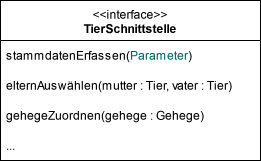
\includegraphics[scale=1.0]{Bilder/Kapitel-8/interface_tier.pdf}
	\caption{Interface \sttpUMLText{Tier}}
	\label{fig:interface_tier}
\end{figure}

\vspace{\baselineskip} %%% für Druck

Abbildung~\ref{fig:interface_tier} zeigt ein Interface für die Tier-Klasse von Seite~\pageref{sec:Kap-8.2:Tierklasse}, das speziell auf die Tätigkeiten zugeschnitten ist, die der Tierpfleger bei der Erfassung neu\-geborener Tiere ausführen soll. In der Operation \sttpUMLText{stammdatenErfassen()} steht in der Abbildung nur ein Platzhalter „Parameter“. Je nachdem, welche der Attribute der Klasse \sttpUMLText{Tier} zu den Stammdaten gezählt werden, können dort unterschiedlich viele Parameter aufgeführt werden. Folgt man der textuellen Beschreibung auf Seite~\pageref{sec:Kap-8.2:Tiererfassung} sind das Name, Größe, Geburtsdatum und Gewicht.

\vspace{\baselineskip} %%% für Druck

\begin{figure}[h!]
	\centering
	\includegraphics[scale=1.0]{Bilder/Kapitel-8/schnittstellen_verwendung.pdf}
	\caption{Schnittstellenverwendung}
	\label{fig:schnittstellen_verwendung}
\end{figure}  

\vspace{\baselineskip} %%% für Druck

Abbildung~\ref{fig:schnittstellen_verwendung} zeigt, wie die Verwendung von Schnittstellen in UML modelliert wird. In dem oberen Teil der Abbildung ist dargestellt, dass die Klasse \sttpUMLText{Tier} das Interface \sttpUMLText{TierSchnittstelle} realisiert. Der untere Teil der Abbildung zeigt die UML-Syntax, wenn eine Dienstnutzerklasse das Interface verwendet, um die entsprechenden Funktionalitäten der Klasse \sttpUMLText{Tier} zu nutzen.




\clearpage
\section{Kommentierte Literatur}
\label{sec:Kap-8.7}



\sttpKommLitItem{Lahres/Raýman/Strich}{2018}{Objektorientierte Programmierung}{lah18}{Bilder/Buchcover/Buchcover_Lahres_Rayman_Strich.png}{}
{Sehr umfassende Behandlung der objektorientierten Programmierung. Die Themen, die wir in Kapitel~\ref{sec:Kap-8} behandelt haben, finden Sie in diesem Buch in den Kapiteln 4 und 5 und dort noch sehr viele Themen mehr. Die Darstellung ist sehr strukturiert und stark konzeptionell ausgerichtet.} 

\sttpKommLitItem{Kecher/Salvanos/Hoffmann-Elbern}{2018}{UML~2.5}{kec18}{Bilder/Buchcover/Buchcover_Kecher_Salvanos.jpg}{}
{Hier finden Sie die komplette Übersicht der Elemente, die man in UML-Klassen\-dia\-gram\-men einsetzen kann. Bei vielen Elementen wird auch kurz thematisiert, für welche Zwecke man sie verwenden kann. Bei manchen ist Beispielcode für die Umsetzung in Java angegeben.}



